\documentclass[a4paper,11pt, uplatex,openany]{jsbook}

%%%% Packages
%\usepackage{fancyhdr}
\usepackage{thesis2017} 

%
%% 以下, 必要ないものは消してください. 
%\usepackage{fancyhdr}
\usepackage{layout} % 第3章中の \layout のためだけなので, 論文執筆には不要. 
\usepackage[dvipdfmx]{hyperref} % 目次をクリックするとそのページに飛ぶ.
\usepackage{pxjahyper} % hyperrefを使った時に文字化けする場合は使う.
\usepackage{amsmath} % 数式扱うなら必須.
\usepackage{ascmac} % 文章の枠囲み. 論文では不要だと思う.  
\usepackage[dvipdfmx]{xcolor} % 文字に色をつける. これも不要. 
\usepackage[dvipdfmx]{graphicx} % 図の挿入に必要. 
\usepackage[skip=5pt]{caption} % あった方がいい. 
\captionsetup{labelfont=bf} % あった方がいい. 
\usepackage[
  labelformat=simple, 
  list=true, 
  listformat=simple]{subcaption} % 図3.2(a)的なことをする場合は必要
  \renewcommand\thesubfigure{(\alph{subfigure})} % 図3.2(a)的なことをする場合は必要
 

%%%% Settings
\bibliographystyle{junsrt}

%%%% \def: Definitions
\def\diff{\mathrm{d}}
\def\BibTeX{B{\small IB}\TeX}



%%%%%%%% Document
\begin{document}

%
%前書き
\frontmatter
\clearpage
% タイトルページ
\begin{titlepage}
\centering
\vspace*{40truept}
{\Large 平成27年度 卒業研究報告書} \\ % 年度
\vspace{40truept} 
 {\Large 題目} \\
 \vspace{10truept} 
{\LARGE \textbf{タイトル}}\\ % タイトル
\vspace{10truept}
{\Large --- サブタイトル ---}\\ % サブタイトル. なければコメントアウト
\vspace{120truept}
{\Large 指導教員}\\ %
 \vspace{10truept} 
{\Large 石川 将人 教授}\\ % 指導教員
\vspace{60truept}
{\Large 大阪大学 工学部 応用理工学科}\\ % 学科
 \vspace{10truept} 
{\Large 学籍番号 08B12***}\\ % 学籍番号
\vspace{20truept}
{\LARGE 名前}\\ % 著者
\vspace{80truept}
{\Large 2016年2月xx日} % 提出日
\end{titlepage}
\cleardoublepage
% アブストラクト
\chapter*{\huge 概要}
\vskip2\Cvs

卒業論文を\LaTeX で書くときに参考になればと思い作りました. なぜかコンパイルできない, Wordみたいな微調整ができなくて体裁が整わないなどの``\LaTeX あるある''で, 無駄に時間を費やさないように, 本来時間を割くべきところにきちんと時間を割けるようにしましょう. 

本テンプレートは使用を強要するものではありません. すでにShareフォルダ内に, 末岡先生が作られた大須賀研用のテンプレがありますのでそれを用いてもらっても構いません. あるいは自分で論文体裁を整えてもらっても構いません. 要するに論文が書ければそれでいいのです. 

本テンプレートは完成度は高くないです. より多くの知識や経験を今後に生かすため, 気がついたことがあれば随時加筆修正を行ってくださると幸いです. また, \chapref{論文の書き方}と\chapref{LaTeX で論文を書くときのノウハウ}に書いてある内容なんかも参考にしてもらえればと思います. 

\begin{table}[h]
\caption*{Specification of this template}
\tablab{Specification of this template}
\centering
\begin{tabular}{ll}\hline\hline
最終更新日 & \today\\\hline
本テンプレート保存場所 & \verb|/knight/share/テンプレート/LaTeX/thesis_utf8|\\\hline
動作確認した\TeX 環境 & TeX Live 2015: ptex2pdf. Mac OSX, Windows7共に確認. \\\hline
\end{tabular}
\end{table}%




\section*{\huge Abstract}
\vskip2\Cvs
This paper discusses ...
%
%


\newpage

%目次
\tableofcontents   %目次
\thispagestyle{plain}
%\newpage
\listoffigures %図目次 図が少なければいらないかも
%\newpage
\listoftables %表目次 表が少なければいらないかも
%\newpage

 %タイトル・概要・目次など

%本文
\mainmatter
\chapter{はじめに}



\section{背景}
世の中にはこんな問題がある. 

\section{本研究の目的・成果の概要}
本研究ではこんなことに取り組んだ. その結果こんな結果がえられた. 

\section{本論文の構成}
本論文の構成は以下の通りである. 
第2章では論文を記述する上での一般的なルールについて述べる. 
第3章では\LaTeX を用いて論文を記述する上でのノウハウについて述べる. 
最後に,第4章で本論文をまとめる.
 %第1章
\chapter{論文の書き方}\chaplab{論文の書き方}
本章では, 論文の書き方についての一般的なルールや重要な点を幾つか挙げる. 

\section{句読点}
句読点は「、」「。」ではなく, 「, 」「. 」を使うのが機械学会のあたりの分野での習慣. 全角の「,」「.」か半角+半角スペース「, 」「. 」はどちらでも良さそうだが, 自分の中で統一して書く. 


\section{文字式は斜体, 単位は立体}
\begin{itembox}[c]{間違い}
  \begin{align}
    x = rθ sinφ \quad [m]
  \end{align}
ここでx[m]は変位, θ[rad]は角度とする. 
\end{itembox}
\addtocounter{equation}{-1}
\begin{itembox}[c]{正しくは}
  \begin{align}
    x = r\theta \sin\phi \quad [\mathrm{m}]
  \end{align}
ここで$x[\mathrm{m}]$は変位, $\theta[\mathrm{rad}]$は角度とする. 

\end{itembox}
数式環境中でメートルの単位が斜体に ($m$),  文章中で文字式が立体 (x) になっている. ついでに言うと, $\theta$, $\phi$が全角文字で変換したもの (θ, φ) になっており, \LaTeX では扱うべきではない. また, 三角関数$\sin$や行列式$\det$など汎用的な数学記号についても立体にする. 
ほげほげ
ほげほげ
ほげほげ
ほげほげ
ほげほげ
ほげほげ
ほげほげ
ほげほげ
ほげほげ
ほげほげ
ほげほげ
ほげほげ
ほげほげ
ほげほげ
ほげほげ
ほげほげ
ほげほげ

\section{引用について}
引用箇所には必ず参考文献の参照ラベルを振る\cite{knuth1986texbook}. こんな感じ. 文章や図のコピペは厳禁. 図については, 基本的に自分で描くようにするべき. \LaTeX では\BibTeX を用いるのが良い. 


\section{グラフについて}
 %第2章
\chapter{\LaTeX で論文を書くときのノウハウ}\chaplab{LaTeX で論文を書くときのノウハウ}
本章では\LaTeX で論文を書くときの...

\addtocounter{section}{-1}
\section{論文を書き始める前に...}
\subsection{\TeX をアップデートしておく}
\TeX Live 2014以降であれば, \TeX 環境をインターネットを通じて手動でアップデートすることができる. tlmgr (TeX Live manager) を使って最新の状態にアップデートしておくのがよい.  
\subsection{本テンプレートが動作した\TeX 環境}
本テンプレートはMac OSX, Windows7 共に動作確認をしている. 
\begin{description}
\item[Mac OSX] TeX Live 2015. ptex2pdfを利用. TeXShopでのコンパイルに成功. 
\item[Windows7] TeX Live 2015. ptex2pdfを利用. TeXworksでのコンパイルに成功. 文字コードはutf8で, Shift JISへの変換の必要はない. 
\end{description}



\section{本テンプレートの余白の設定}
\begin{itemize}
\item 紙ファイルに卒論を綴じること前提で設定しているので注意
\item 紙ファイルの綴じ幅: 18mm = 51pt
\item 綴じ幅を除いた範囲の上左右下の余白: \{25mm, 20mm, 20mm, 20mm\} = \{1inch(72pt), 57pt, 57pt, 57pt\}
\item header, margin note は使わないのが前提. footerはページ番号にのみ使う
\end{itemize}
%\vspace{15pt}

%\layout
%\newpage
 
\section{卒論データを整理して保存}
卒論のような非常に大規模な文章を\LaTeX で書く場合, それに伴って使用する画像は非常に多くなる. これを\verb|main.tex|と同じ場所に保存すると, 可視性が悪い上に整理も難しくなり, 作業効率も悪くなる. さらに, \verb|main.tex|に全ての文章や数式を書き切ろうとすると, 何千何万行と言う膨大なソースファイルとなり, やはり扱いづらくなる. そこで, \verb|\input|コマンドやファイルの相対パス指定をうまく使い, データを整理することが望ましい. 

\begin{figure}[htbp]
  \centering
  \fbox{
    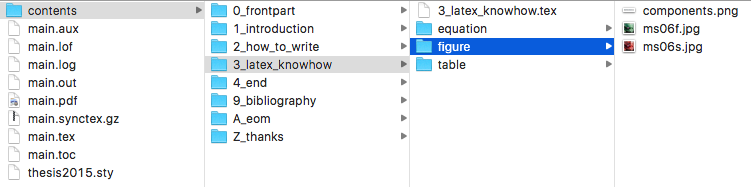
\includegraphics[width=.9\textwidth]{./contents/3_latex_knowhow/figure/components.png}
  }
  \caption{Components of the thesis directry}
  \figlab{components.png}
\end{figure}

\figref{components.png}に本テンプレートにおける論文データの構成を示す. \verb|main.tex|と同じディレクトリ内に\verb|contents|という名前のディレクトリが存在し, その中に各章ごとのデータが存在する. 各章のディレクトリ内には, その章のドキュメントのtexデータと, 付随するtexデータや画像データなどが存在する. 以下, この論文データの構成でどのようにtexソースファイルを記述するかについて説明する. 

\textbackslash input コマンドは, 挿入用に用意したtexソースファイルを挿入したい場所に挿入するコマンドである. 
例えば, \verb|main.tex| 内には
\verb|\chapter{\LaTeX で論文を書くときのノウハウ}\chaplab{LaTeX で論文を書くときのノウハウ}
本章では\LaTeX で論文を書くときの...

\addtocounter{section}{-1}
\section{論文を書き始める前に...}
\subsection{\TeX をアップデートしておく}
\TeX Live 2014以降であれば, \TeX 環境をインターネットを通じて手動でアップデートすることができる. tlmgr (TeX Live manager) を使って最新の状態にアップデートしておくのがよい.  
\subsection{本テンプレートが動作した\TeX 環境}
本テンプレートはMac OSX, Windows7 共に動作確認をしている. 
\begin{description}
\item[Mac OSX] TeX Live 2015. ptex2pdfを利用. TeXShopでのコンパイルに成功. 
\item[Windows7] TeX Live 2015. ptex2pdfを利用. TeXworksでのコンパイルに成功. 文字コードはutf8で, Shift JISへの変換の必要はない. 
\end{description}



\section{本テンプレートの余白の設定}
\begin{itemize}
\item 紙ファイルに卒論を綴じること前提で設定しているので注意
\item 紙ファイルの綴じ幅: 18mm = 51pt
\item 綴じ幅を除いた範囲の上左右下の余白: \{25mm, 20mm, 20mm, 20mm\} = \{1inch(72pt), 57pt, 57pt, 57pt\}
\item header, margin note は使わないのが前提. footerはページ番号にのみ使う
\end{itemize}
%\vspace{15pt}

%\layout
%\newpage
 
\section{卒論データを整理して保存}
卒論のような非常に大規模な文章を\LaTeX で書く場合, それに伴って使用する画像は非常に多くなる. これを\verb|main.tex|と同じ場所に保存すると, 可視性が悪い上に整理も難しくなり, 作業効率も悪くなる. さらに, \verb|main.tex|に全ての文章や数式を書き切ろうとすると, 何千何万行と言う膨大なソースファイルとなり, やはり扱いづらくなる. そこで, \verb|\input|コマンドやファイルの相対パス指定をうまく使い, データを整理することが望ましい. 

\begin{figure}[htbp]
  \centering
  \fbox{
    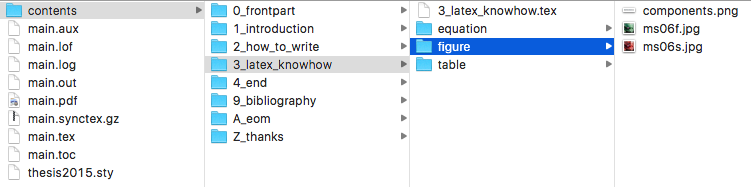
\includegraphics[width=.9\textwidth]{./contents/3_latex_knowhow/figure/components.png}
  }
  \caption{Components of the thesis directry}
  \figlab{components.png}
\end{figure}

\figref{components.png}に本テンプレートにおける論文データの構成を示す. \verb|main.tex|と同じディレクトリ内に\verb|contents|という名前のディレクトリが存在し, その中に各章ごとのデータが存在する. 各章のディレクトリ内には, その章のドキュメントのtexデータと, 付随するtexデータや画像データなどが存在する. 以下, この論文データの構成でどのようにtexソースファイルを記述するかについて説明する. 

\textbackslash input コマンドは, 挿入用に用意したtexソースファイルを挿入したい場所に挿入するコマンドである. 
例えば, \verb|main.tex| 内には
\verb|\chapter{\LaTeX で論文を書くときのノウハウ}\chaplab{LaTeX で論文を書くときのノウハウ}
本章では\LaTeX で論文を書くときの...

\addtocounter{section}{-1}
\section{論文を書き始める前に...}
\subsection{\TeX をアップデートしておく}
\TeX Live 2014以降であれば, \TeX 環境をインターネットを通じて手動でアップデートすることができる. tlmgr (TeX Live manager) を使って最新の状態にアップデートしておくのがよい.  
\subsection{本テンプレートが動作した\TeX 環境}
本テンプレートはMac OSX, Windows7 共に動作確認をしている. 
\begin{description}
\item[Mac OSX] TeX Live 2015. ptex2pdfを利用. TeXShopでのコンパイルに成功. 
\item[Windows7] TeX Live 2015. ptex2pdfを利用. TeXworksでのコンパイルに成功. 文字コードはutf8で, Shift JISへの変換の必要はない. 
\end{description}



\section{本テンプレートの余白の設定}
\begin{itemize}
\item 紙ファイルに卒論を綴じること前提で設定しているので注意
\item 紙ファイルの綴じ幅: 18mm = 51pt
\item 綴じ幅を除いた範囲の上左右下の余白: \{25mm, 20mm, 20mm, 20mm\} = \{1inch(72pt), 57pt, 57pt, 57pt\}
\item header, margin note は使わないのが前提. footerはページ番号にのみ使う
\end{itemize}
%\vspace{15pt}

%\layout
%\newpage
 
\section{卒論データを整理して保存}
卒論のような非常に大規模な文章を\LaTeX で書く場合, それに伴って使用する画像は非常に多くなる. これを\verb|main.tex|と同じ場所に保存すると, 可視性が悪い上に整理も難しくなり, 作業効率も悪くなる. さらに, \verb|main.tex|に全ての文章や数式を書き切ろうとすると, 何千何万行と言う膨大なソースファイルとなり, やはり扱いづらくなる. そこで, \verb|\input|コマンドやファイルの相対パス指定をうまく使い, データを整理することが望ましい. 

\begin{figure}[htbp]
  \centering
  \fbox{
    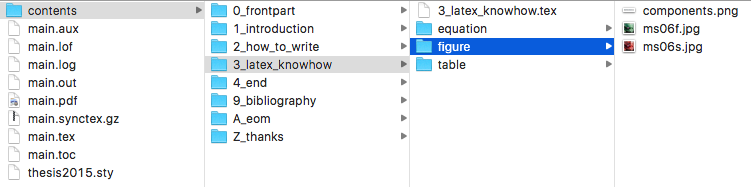
\includegraphics[width=.9\textwidth]{./contents/3_latex_knowhow/figure/components.png}
  }
  \caption{Components of the thesis directry}
  \figlab{components.png}
\end{figure}

\figref{components.png}に本テンプレートにおける論文データの構成を示す. \verb|main.tex|と同じディレクトリ内に\verb|contents|という名前のディレクトリが存在し, その中に各章ごとのデータが存在する. 各章のディレクトリ内には, その章のドキュメントのtexデータと, 付随するtexデータや画像データなどが存在する. 以下, この論文データの構成でどのようにtexソースファイルを記述するかについて説明する. 

\textbackslash input コマンドは, 挿入用に用意したtexソースファイルを挿入したい場所に挿入するコマンドである. 
例えば, \verb|main.tex| 内には
\verb|\input{./contents/3_latex_knowhow/3_latex_knowhow.tex}| 
が記述されている. ここで, \verb|./contents/3_latex_knowhow/3_latex_knowhow.tex|は挿入するtexソースファイルを指定する相対パスである. 

このコマンドについて具体的に説明する. \verb|main.tex|に\figref{components.png}中の左から3段目にある``\verb|3_latex_knowhow.tex|''を挿入している. ``\verb|./|''は \verb|main.tex| が存在するディレクトリを, ``\verb|contents/|''はその中にある``\verb|contents|''というディレクトリの名前を, ``\verb|3_latex_knowhow/|''はさらにその中にある``\verb|3_latex_knowhow|''というディレクトリの名前を, そして最後の``\verb|3_latex_knowhow.tex|''はその中にある``\verb|3_latex_knowhow.tex|''を指している\footnote{
拡張子 ``.tex'' は省略して書くこともできる. 
}. このように, \textbackslash input コマンドと相対パスの指定をうまく組み合わせることで, 論文データを整理して扱うことができる. 

画像のパスも同様に指定することができる. 例えば\figref{components.png}は, \\
\verb|\includegraphics[width=.9\textwidth]|\\
\verb|{./contents/3_latex_knowhow/figure/components.png}|\\
のようにして画像データを指定している\footnote{
これも拡張子は省略できる. ただし, 同名別拡張子のファイルを読み込む可能性があるため, 注意が必要. 
}. 

さらに, 表や規模の大きな数式など, 数十〜数百行に渡る一括りのソースは, \textbackslash input コマンドを積極的に使用することで, ソースファイルを整理することができる. 本テンプレートでは例えば\figref{Example of writing a table}や\tabref{Title}でこれを用いている. 


\section{図・表の副番号 (\figref{ms06f.jpg}的なもの)}
例えば\figref{ZAKU}のようにする
\footnote{同様のことを実現するためにsubfigure.styやsubfig.styを用いた例が多く存在する. 思い通りに出力できるのであればもちろんこれでも良いが, 上述のパッケージは開発が中止されているため, また他のパッケージとの互換性や設定の自由度などからcaption.styとsubcaption.styで実現するのが良いと思われる. }. 

\begin{figure}[h]
  \begin{minipage}[b]{.5\textwidth}
    \centering
    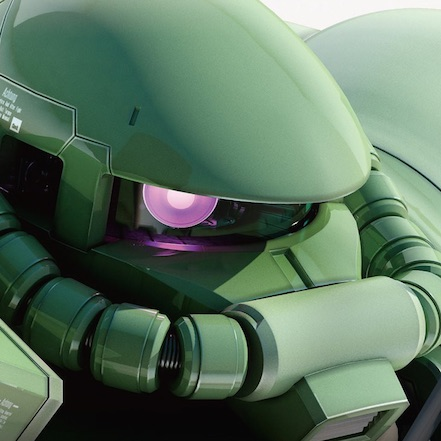
\includegraphics[width=.9\textwidth]{./contents/3_latex_knowhow/figure/ms06f.jpg}
    \subcaption{MS06F}\figlab{ms06f.jpg}
  \end{minipage}%
  \begin{minipage}[b]{.5\textwidth}
    \centering
    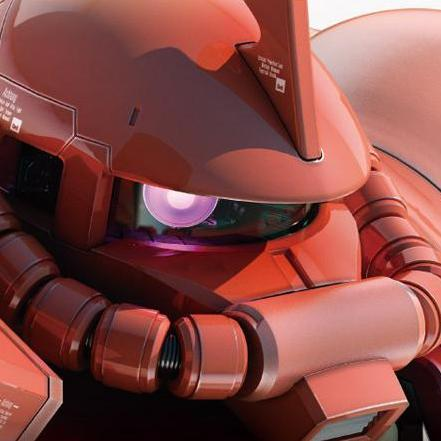
\includegraphics[width=.9\textwidth]{./contents/3_latex_knowhow/figure/ms06s.jpg}
    \subcaption{MS06S}\figlab{ms06s.jpg}
  \end{minipage}
  \caption{ZAKU}\figlab{ZAKU}
\end{figure}


\section{通し番号について (\textbackslash label, \textbackslash ref, 及びこれらを用いた応用)}
\subsection{本文中での通し番号の直書きは厳禁!}
\LaTeX では, 図, 表, 数式, 章や節など, ページ番号で自動的に番号が振られる. 例えば
\begin{screen}
\begin{verbatim} 
\begin{figure}
  \centering
  \includegraphics{figure.png}
  \caption{caption title}
\end{figure}
\end{verbatim}
\end{screen}
とすることで, \verb|\caption| の部分で自動的に番号が振られる. この番号は参照をすることが可能である. すなわち, 上述の結果図のキャプションが``\textbf{Fig.~1}:~caption title''となった場合, ソースファイルに``\verb|\textbf{Fig.~1}に示すように|...''といったように, 具体的な図番号を書かず, 番号を自動的に挿入することができるようにすることができる. と言うより, 執筆途中に図を挟み込むことが多々あるうえに扱う通し番号が沢山ある\LaTeX 文章においてはむしろ, 図番号をソースファイルに直接書くべきではない. 

\subsection{\textbackslash label, \textbackslash ref について}
例えば図や表の場合, 
\begin{screen}
\begin{verbatim} 
\begin{figure}
  \centering
  \includegraphics{figure.png}
  \caption{caption title}
  \label{figure label}
\end{figure}
\end{verbatim}
\end{screen}
のように, \verb|\caption{}|の直後に\verb|\label{}|を記述することで, 本文中で
\begin{screen}
\verb|\textbf{Fig.~\ref{figure label}}|に示すように...
\end{screen}
と書けば``\textbf{Fig.~1}に示すように...''と表示される. 

\subsection{\textbackslash figlab, \textbackslash figref などの応用}
これで通し番号の参照が可能なのだが, \verb|\textbf{Fig.~|...\verb|}|の部分も省略することができる. 詳細な説明は割愛するが, \verb|thesis2015.sty|中で
\begin{itembox}[c]{プリアンブル}
\begin{verbatim} 
\renewcommand{\figurename}{Fig.}
\def\figlab#1{\label{fig:#1}}
\def\figref#1{\textbf{\figurename~\ref{fig:#1}}}
\end{verbatim}
\end{itembox}
が定義されており, 
\begin{itembox}[c]{本文}
\begin{verbatim} 
\begin{figure}
  \centering
  \includegraphics{figure.png}
  \caption{caption title}
  \figlab{figure label}
\end{figure}
\end{verbatim}
\end{itembox}
とすることで, 
\begin{itembox}[c]{本文}
\begin{verbatim} 
\verb|\figref{figure label}|に示すように...
\end{verbatim}
\end{itembox}
と書けば同様の結果が得られるようになっている. 

同様に使えるコマンドとして, \verb|\tablab|, \verb|\tabref|, \verb|\eqnlab|, \verb|\eqnref|, \verb|\chaplab|, \verb|\chapref|, \verb|\seclab|, \verb|\secref|, \verb|\subseclzab|, \verb|\subsecref|が定義されている. 

\section{表の作成について}
Excelを使うと便利かも. \figref{Example of writing a table}にその例を示す. 


\input{./contents/3_latex_knowhow/text/example_of_writing_a_table}
\input{./contents/3_latex_knowhow/text/sample_table}


\section{参考文献について: \BibTeX を使う}
卒論のみならず, 今後月報や投稿論文, 予稿などを書く際にも参考文献は何度も記述することになる. そこで, 「参考文献リスト」であるbibファイルを作り, \BibTeX を使うことでその管理が非常にやりやすくなる. bibファイルは, TeXShop やTeXworks などとは別のエディター (BibDesk (Mac)など) が必要です. 


\section{検索・置換機能を使う}
\LaTeX に限った話ではないが, 「control + F」(Windows) や「command + F」(Mac) で文書内の文字列を検索したり別の文字列への置換を行うことが可能である. 例えば間違って書いた複数の「、」を「, 」に修正するときなどに. 


\section{ソースファイルに書いてる記述に間違いないはずなのにコンパイルできない}
一度\verb|main.tex|と同じ場所に生成されている\verb|main.aux|を消してからもう一度コンパイルしてみてください.  


\section{通し番号が反映されない / \BibTeX の内容が反映されない}
通し番号を反映するためには2回コンパイルする必要があります. \BibTeX に関しては, \LaTeX$\rightarrow$\BibTeX$\rightarrow$\LaTeX$\rightarrow$\LaTeX で計4回のコンパイルが必要です. 

| 
が記述されている. ここで, \verb|./contents/3_latex_knowhow/3_latex_knowhow.tex|は挿入するtexソースファイルを指定する相対パスである. 

このコマンドについて具体的に説明する. \verb|main.tex|に\figref{components.png}中の左から3段目にある``\verb|3_latex_knowhow.tex|''を挿入している. ``\verb|./|''は \verb|main.tex| が存在するディレクトリを, ``\verb|contents/|''はその中にある``\verb|contents|''というディレクトリの名前を, ``\verb|3_latex_knowhow/|''はさらにその中にある``\verb|3_latex_knowhow|''というディレクトリの名前を, そして最後の``\verb|3_latex_knowhow.tex|''はその中にある``\verb|3_latex_knowhow.tex|''を指している\footnote{
拡張子 ``.tex'' は省略して書くこともできる. 
}. このように, \textbackslash input コマンドと相対パスの指定をうまく組み合わせることで, 論文データを整理して扱うことができる. 

画像のパスも同様に指定することができる. 例えば\figref{components.png}は, \\
\verb|\includegraphics[width=.9\textwidth]|\\
\verb|{./contents/3_latex_knowhow/figure/components.png}|\\
のようにして画像データを指定している\footnote{
これも拡張子は省略できる. ただし, 同名別拡張子のファイルを読み込む可能性があるため, 注意が必要. 
}. 

さらに, 表や規模の大きな数式など, 数十〜数百行に渡る一括りのソースは, \textbackslash input コマンドを積極的に使用することで, ソースファイルを整理することができる. 本テンプレートでは例えば\figref{Example of writing a table}や\tabref{Title}でこれを用いている. 


\section{図・表の副番号 (\figref{ms06f.jpg}的なもの)}
例えば\figref{ZAKU}のようにする
\footnote{同様のことを実現するためにsubfigure.styやsubfig.styを用いた例が多く存在する. 思い通りに出力できるのであればもちろんこれでも良いが, 上述のパッケージは開発が中止されているため, また他のパッケージとの互換性や設定の自由度などからcaption.styとsubcaption.styで実現するのが良いと思われる. }. 

\begin{figure}[h]
  \begin{minipage}[b]{.5\textwidth}
    \centering
    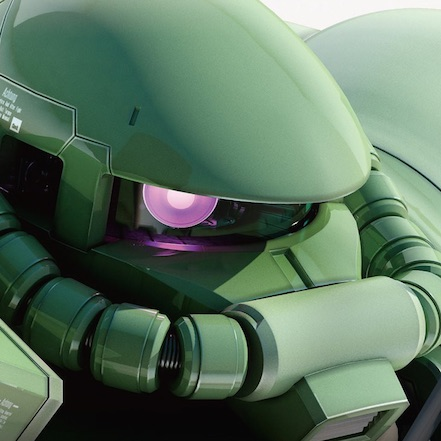
\includegraphics[width=.9\textwidth]{./contents/3_latex_knowhow/figure/ms06f.jpg}
    \subcaption{MS06F}\figlab{ms06f.jpg}
  \end{minipage}%
  \begin{minipage}[b]{.5\textwidth}
    \centering
    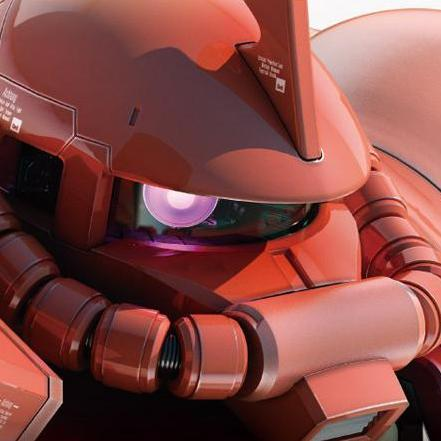
\includegraphics[width=.9\textwidth]{./contents/3_latex_knowhow/figure/ms06s.jpg}
    \subcaption{MS06S}\figlab{ms06s.jpg}
  \end{minipage}
  \caption{ZAKU}\figlab{ZAKU}
\end{figure}


\section{通し番号について (\textbackslash label, \textbackslash ref, 及びこれらを用いた応用)}
\subsection{本文中での通し番号の直書きは厳禁!}
\LaTeX では, 図, 表, 数式, 章や節など, ページ番号で自動的に番号が振られる. 例えば
\begin{screen}
\begin{verbatim} 
\begin{figure}
  \centering
  \includegraphics{figure.png}
  \caption{caption title}
\end{figure}
\end{verbatim}
\end{screen}
とすることで, \verb|\caption| の部分で自動的に番号が振られる. この番号は参照をすることが可能である. すなわち, 上述の結果図のキャプションが``\textbf{Fig.~1}:~caption title''となった場合, ソースファイルに``\verb|\textbf{Fig.~1}に示すように|...''といったように, 具体的な図番号を書かず, 番号を自動的に挿入することができるようにすることができる. と言うより, 執筆途中に図を挟み込むことが多々あるうえに扱う通し番号が沢山ある\LaTeX 文章においてはむしろ, 図番号をソースファイルに直接書くべきではない. 

\subsection{\textbackslash label, \textbackslash ref について}
例えば図や表の場合, 
\begin{screen}
\begin{verbatim} 
\begin{figure}
  \centering
  \includegraphics{figure.png}
  \caption{caption title}
  \label{figure label}
\end{figure}
\end{verbatim}
\end{screen}
のように, \verb|\caption{}|の直後に\verb|\label{}|を記述することで, 本文中で
\begin{screen}
\verb|\textbf{Fig.~\ref{figure label}}|に示すように...
\end{screen}
と書けば``\textbf{Fig.~1}に示すように...''と表示される. 

\subsection{\textbackslash figlab, \textbackslash figref などの応用}
これで通し番号の参照が可能なのだが, \verb|\textbf{Fig.~|...\verb|}|の部分も省略することができる. 詳細な説明は割愛するが, \verb|thesis2015.sty|中で
\begin{itembox}[c]{プリアンブル}
\begin{verbatim} 
\renewcommand{\figurename}{Fig.}
\def\figlab#1{\label{fig:#1}}
\def\figref#1{\textbf{\figurename~\ref{fig:#1}}}
\end{verbatim}
\end{itembox}
が定義されており, 
\begin{itembox}[c]{本文}
\begin{verbatim} 
\begin{figure}
  \centering
  \includegraphics{figure.png}
  \caption{caption title}
  \figlab{figure label}
\end{figure}
\end{verbatim}
\end{itembox}
とすることで, 
\begin{itembox}[c]{本文}
\begin{verbatim} 
\verb|\figref{figure label}|に示すように...
\end{verbatim}
\end{itembox}
と書けば同様の結果が得られるようになっている. 

同様に使えるコマンドとして, \verb|\tablab|, \verb|\tabref|, \verb|\eqnlab|, \verb|\eqnref|, \verb|\chaplab|, \verb|\chapref|, \verb|\seclab|, \verb|\secref|, \verb|\subseclzab|, \verb|\subsecref|が定義されている. 

\section{表の作成について}
Excelを使うと便利かも. \figref{Example of writing a table}にその例を示す. 


\begin{figure}[h]
  \begin{minipage}{\textwidth}
    \centering
    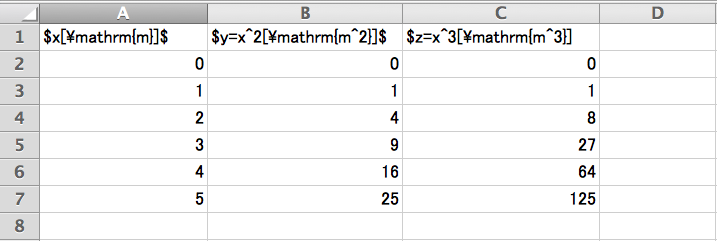
\includegraphics[height=.2\textwidth]{./contents/3_latex_knowhow/figure/table_writing_1.png}
    \subcaption{Write a table you want to write on Excel}\figlab{table_writing_1.png}
    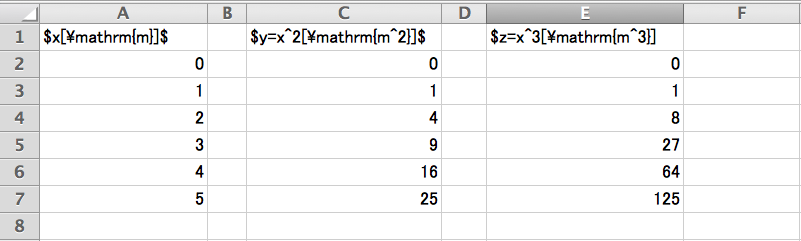
\includegraphics[height=.2\textwidth]{./contents/3_latex_knowhow/figure/table_writing_2.png}
    \subcaption{Add blank columns within each column}\figlab{table_writing_2.png}
    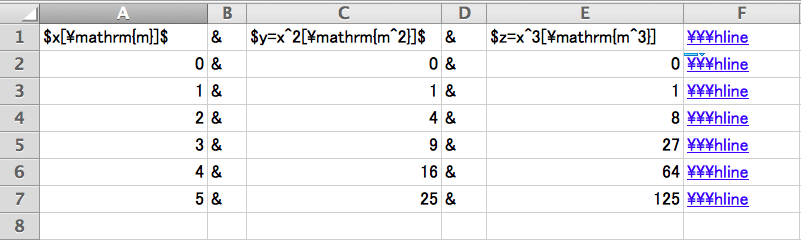
\includegraphics[height=.2\textwidth]{./contents/3_latex_knowhow/figure/table_writing_3.png}
    \subcaption{Fill \& \!s in the blanks column and \textbackslash\textbackslash\textbackslash hline in the last column}\figlab{table_writing_3.png}
    \begin{minipage}{.6\textwidth}
      \begin{screen}
        \centering
        \small{
        \begin{verbatim} 
\begin{table}[htbp]
\centering
\caption{Title}
\tablab{Title}
\begin{tabular}{ l | c | r } \hline\hline
   **here**
\end{tabular}
\end{table}\end{verbatim}}
      \end{screen}
    \end{minipage}
    \subcaption{Copy and paste the table area into **here**}\figlab{table_writing_4}
  \end{minipage}
  \caption{Example of writing \tabref{Title}}\figlab{Example of writing a table}
\end{figure}
\begin{table}[h]
\centering
\caption{Title}
\tablab{Title}
\begin{tabular}{| l | c | r |}\hline
$x[\mathrm{m}]$	&	$y=x^2[\mathrm{m^2}]$	&	$z=x^3[\mathrm{m^3}]	$\\\hline
0	&	0	&	0	\\\hline
1	&	1	&	1	\\\hline
2	&	4	&	8	\\\hline
3	&	9	&	27	\\\hline
4	&	16	&	64	\\\hline
5	&	25	&	125	\\\hline
\end{tabular}
\end{table}


\section{参考文献について: \BibTeX を使う}
卒論のみならず, 今後月報や投稿論文, 予稿などを書く際にも参考文献は何度も記述することになる. そこで, 「参考文献リスト」であるbibファイルを作り, \BibTeX を使うことでその管理が非常にやりやすくなる. bibファイルは, TeXShop やTeXworks などとは別のエディター (BibDesk (Mac)など) が必要です. 


\section{検索・置換機能を使う}
\LaTeX に限った話ではないが, 「control + F」(Windows) や「command + F」(Mac) で文書内の文字列を検索したり別の文字列への置換を行うことが可能である. 例えば間違って書いた複数の「、」を「, 」に修正するときなどに. 


\section{ソースファイルに書いてる記述に間違いないはずなのにコンパイルできない}
一度\verb|main.tex|と同じ場所に生成されている\verb|main.aux|を消してからもう一度コンパイルしてみてください.  


\section{通し番号が反映されない / \BibTeX の内容が反映されない}
通し番号を反映するためには2回コンパイルする必要があります. \BibTeX に関しては, \LaTeX$\rightarrow$\BibTeX$\rightarrow$\LaTeX$\rightarrow$\LaTeX で計4回のコンパイルが必要です. 

| 
が記述されている. ここで, \verb|./contents/3_latex_knowhow/3_latex_knowhow.tex|は挿入するtexソースファイルを指定する相対パスである. 

このコマンドについて具体的に説明する. \verb|main.tex|に\figref{components.png}中の左から3段目にある``\verb|3_latex_knowhow.tex|''を挿入している. ``\verb|./|''は \verb|main.tex| が存在するディレクトリを, ``\verb|contents/|''はその中にある``\verb|contents|''というディレクトリの名前を, ``\verb|3_latex_knowhow/|''はさらにその中にある``\verb|3_latex_knowhow|''というディレクトリの名前を, そして最後の``\verb|3_latex_knowhow.tex|''はその中にある``\verb|3_latex_knowhow.tex|''を指している\footnote{
拡張子 ``.tex'' は省略して書くこともできる. 
}. このように, \textbackslash input コマンドと相対パスの指定をうまく組み合わせることで, 論文データを整理して扱うことができる. 

画像のパスも同様に指定することができる. 例えば\figref{components.png}は, \\
\verb|\includegraphics[width=.9\textwidth]|\\
\verb|{./contents/3_latex_knowhow/figure/components.png}|\\
のようにして画像データを指定している\footnote{
これも拡張子は省略できる. ただし, 同名別拡張子のファイルを読み込む可能性があるため, 注意が必要. 
}. 

さらに, 表や規模の大きな数式など, 数十〜数百行に渡る一括りのソースは, \textbackslash input コマンドを積極的に使用することで, ソースファイルを整理することができる. 本テンプレートでは例えば\figref{Example of writing a table}や\tabref{Title}でこれを用いている. 


\section{図・表の副番号 (\figref{ms06f.jpg}的なもの)}
例えば\figref{ZAKU}のようにする
\footnote{同様のことを実現するためにsubfigure.styやsubfig.styを用いた例が多く存在する. 思い通りに出力できるのであればもちろんこれでも良いが, 上述のパッケージは開発が中止されているため, また他のパッケージとの互換性や設定の自由度などからcaption.styとsubcaption.styで実現するのが良いと思われる. }. 

\begin{figure}[h]
  \begin{minipage}[b]{.5\textwidth}
    \centering
    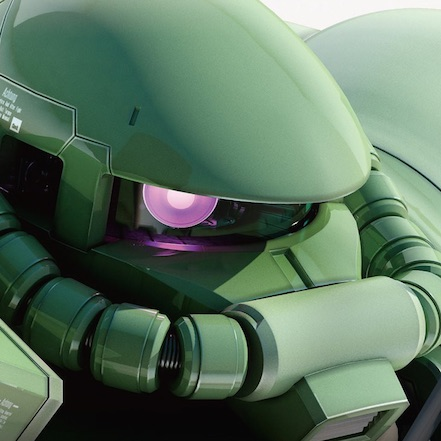
\includegraphics[width=.9\textwidth]{./contents/3_latex_knowhow/figure/ms06f.jpg}
    \subcaption{MS06F}\figlab{ms06f.jpg}
  \end{minipage}%
  \begin{minipage}[b]{.5\textwidth}
    \centering
    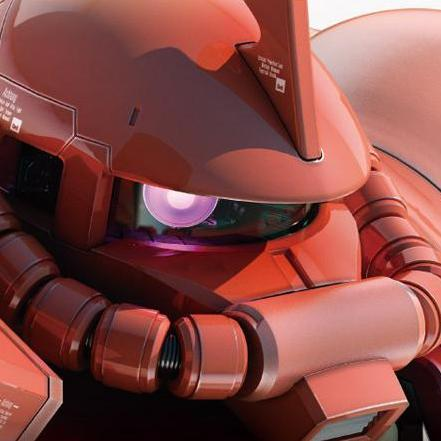
\includegraphics[width=.9\textwidth]{./contents/3_latex_knowhow/figure/ms06s.jpg}
    \subcaption{MS06S}\figlab{ms06s.jpg}
  \end{minipage}
  \caption{ZAKU}\figlab{ZAKU}
\end{figure}


\section{通し番号について (\textbackslash label, \textbackslash ref, 及びこれらを用いた応用)}
\subsection{本文中での通し番号の直書きは厳禁!}
\LaTeX では, 図, 表, 数式, 章や節など, ページ番号で自動的に番号が振られる. 例えば
\begin{screen}
\begin{verbatim} 
\begin{figure}
  \centering
  \includegraphics{figure.png}
  \caption{caption title}
\end{figure}
\end{verbatim}
\end{screen}
とすることで, \verb|\caption| の部分で自動的に番号が振られる. この番号は参照をすることが可能である. すなわち, 上述の結果図のキャプションが``\textbf{Fig.~1}:~caption title''となった場合, ソースファイルに``\verb|\textbf{Fig.~1}に示すように|...''といったように, 具体的な図番号を書かず, 番号を自動的に挿入することができるようにすることができる. と言うより, 執筆途中に図を挟み込むことが多々あるうえに扱う通し番号が沢山ある\LaTeX 文章においてはむしろ, 図番号をソースファイルに直接書くべきではない. 

\subsection{\textbackslash label, \textbackslash ref について}
例えば図や表の場合, 
\begin{screen}
\begin{verbatim} 
\begin{figure}
  \centering
  \includegraphics{figure.png}
  \caption{caption title}
  \label{figure label}
\end{figure}
\end{verbatim}
\end{screen}
のように, \verb|\caption{}|の直後に\verb|\label{}|を記述することで, 本文中で
\begin{screen}
\verb|\textbf{Fig.~\ref{figure label}}|に示すように...
\end{screen}
と書けば``\textbf{Fig.~1}に示すように...''と表示される. 

\subsection{\textbackslash figlab, \textbackslash figref などの応用}
これで通し番号の参照が可能なのだが, \verb|\textbf{Fig.~|...\verb|}|の部分も省略することができる. 詳細な説明は割愛するが, \verb|thesis2015.sty|中で
\begin{itembox}[c]{プリアンブル}
\begin{verbatim} 
\renewcommand{\figurename}{Fig.}
\def\figlab#1{\label{fig:#1}}
\def\figref#1{\textbf{\figurename~\ref{fig:#1}}}
\end{verbatim}
\end{itembox}
が定義されており, 
\begin{itembox}[c]{本文}
\begin{verbatim} 
\begin{figure}
  \centering
  \includegraphics{figure.png}
  \caption{caption title}
  \figlab{figure label}
\end{figure}
\end{verbatim}
\end{itembox}
とすることで, 
\begin{itembox}[c]{本文}
\begin{verbatim} 
\verb|\figref{figure label}|に示すように...
\end{verbatim}
\end{itembox}
と書けば同様の結果が得られるようになっている. 

同様に使えるコマンドとして, \verb|\tablab|, \verb|\tabref|, \verb|\eqnlab|, \verb|\eqnref|, \verb|\chaplab|, \verb|\chapref|, \verb|\seclab|, \verb|\secref|, \verb|\subseclzab|, \verb|\subsecref|が定義されている. 

\section{表の作成について}
Excelを使うと便利かも. \figref{Example of writing a table}にその例を示す. 


\begin{figure}[h]
  \begin{minipage}{\textwidth}
    \centering
    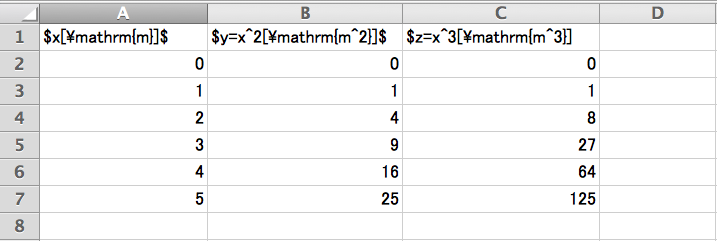
\includegraphics[height=.2\textwidth]{./contents/3_latex_knowhow/figure/table_writing_1.png}
    \subcaption{Write a table you want to write on Excel}\figlab{table_writing_1.png}
    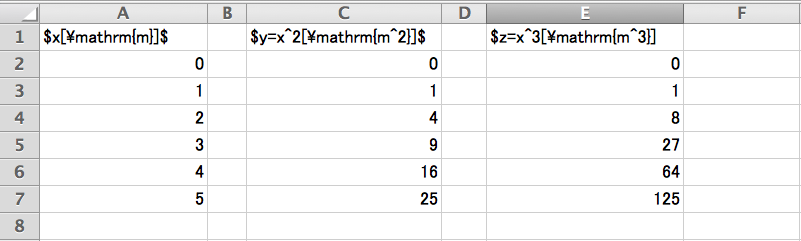
\includegraphics[height=.2\textwidth]{./contents/3_latex_knowhow/figure/table_writing_2.png}
    \subcaption{Add blank columns within each column}\figlab{table_writing_2.png}
    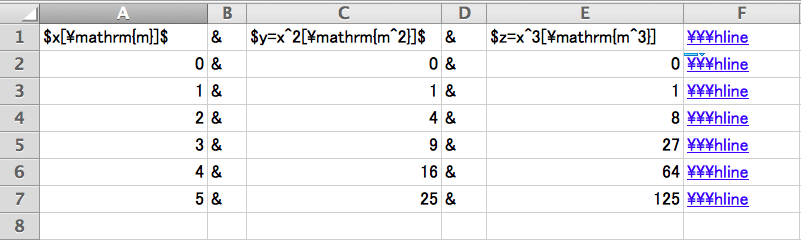
\includegraphics[height=.2\textwidth]{./contents/3_latex_knowhow/figure/table_writing_3.png}
    \subcaption{Fill \& \!s in the blanks column and \textbackslash\textbackslash\textbackslash hline in the last column}\figlab{table_writing_3.png}
    \begin{minipage}{.6\textwidth}
      \begin{screen}
        \centering
        \small{
        \begin{verbatim} 
\begin{table}[htbp]
\centering
\caption{Title}
\tablab{Title}
\begin{tabular}{ l | c | r } \hline\hline
   **here**
\end{tabular}
\end{table}\end{verbatim}}
      \end{screen}
    \end{minipage}
    \subcaption{Copy and paste the table area into **here**}\figlab{table_writing_4}
  \end{minipage}
  \caption{Example of writing \tabref{Title}}\figlab{Example of writing a table}
\end{figure}
\begin{table}[h]
\centering
\caption{Title}
\tablab{Title}
\begin{tabular}{| l | c | r |}\hline
$x[\mathrm{m}]$	&	$y=x^2[\mathrm{m^2}]$	&	$z=x^3[\mathrm{m^3}]	$\\\hline
0	&	0	&	0	\\\hline
1	&	1	&	1	\\\hline
2	&	4	&	8	\\\hline
3	&	9	&	27	\\\hline
4	&	16	&	64	\\\hline
5	&	25	&	125	\\\hline
\end{tabular}
\end{table}


\section{参考文献について: \BibTeX を使う}
卒論のみならず, 今後月報や投稿論文, 予稿などを書く際にも参考文献は何度も記述することになる. そこで, 「参考文献リスト」であるbibファイルを作り, \BibTeX を使うことでその管理が非常にやりやすくなる. bibファイルは, TeXShop やTeXworks などとは別のエディター (BibDesk (Mac)など) が必要です. 


\section{検索・置換機能を使う}
\LaTeX に限った話ではないが, 「control + F」(Windows) や「command + F」(Mac) で文書内の文字列を検索したり別の文字列への置換を行うことが可能である. 例えば間違って書いた複数の「、」を「, 」に修正するときなどに. 


\section{ソースファイルに書いてる記述に間違いないはずなのにコンパイルできない}
一度\verb|main.tex|と同じ場所に生成されている\verb|main.aux|を消してからもう一度コンパイルしてみてください.  


\section{通し番号が反映されない / \BibTeX の内容が反映されない}
通し番号を反映するためには2回コンパイルする必要があります. \BibTeX に関しては, \LaTeX$\rightarrow$\BibTeX$\rightarrow$\LaTeX$\rightarrow$\LaTeX で計4回のコンパイルが必要です. 

 %第3章
\chapter{おわりに}
本論文ではxxxついて議論した. 
得られた主な結果は以下の通りである. 
\begin{itemize}
 \item xxx
 \item xxx
\end{itemize}

今後はxxxする. 

\begin{center}
\color{red}{\Large \textgt{卒論頑張ってください!!!}}
\end{center} %第4章

% 参考文献
\bibliography{ref}

%\begin{thebibliography}{99}% 文献が10以上のとき99,10未満のとき9
%\bibitem{Yoshikawa}
%{苗字, 苗字}:
%``タイトル'',
%雑誌名,vol.13, no.7, pp.994--1005, 1995.
%\end{thebibliography} %参考文献

%付録
\appendix
\chapter{運動方程式の導出}

付録があればこんな感じで書く.  %付録A

%
%後書き
\backmatter
%謝辞
%%%%%%%
% 謝辞
%%%%%%%
\chapter{謝辞}

本論文をまとめるにあたり, 数多くの助言, 提案, 活発な議論をしていただいた石川将人教授に心から感謝申し上げます. また, 研究を進める際に様々な御助言, ご協力をいただきました石川研究室の皆様に心から感謝いたします.

みたいに大体の人は真面目に書きます. ちなみに過去には天津麻婆丼や栄養ドリンクに謝辞を述べた先輩もいたそうです(笑). 



\end{document}
